\documentclass[11pt]{article}
\author{Tarang Srivastava}
\usepackage{amsmath, amsthm}
\usepackage{graphicx}
\usepackage{multicol}
\usepackage{esdiff}
\usepackage[margin=.25in]{geometry}
\geometry{letterpaper,textwidth=7.3in,hmarginratio=1:1,	textheight=9in,vmarginratio=1:1,heightrounded}
\newcommand{\makechaptertitle}[1]{
\begin{center}
	\begin{large}
		DECA Chapter #1 Test
	\end{large}
	\begin{small}
		\\by Tarang Srivastava
	\end{small}
\end{center}
}
\theoremstyle{definition}
\newtheorem{q}{}
\begin{document}
	\begin{multicols*}{2}
		\makechaptertitle{7}
		\begin{q}
			Find the general solution of the system \[ \textbf{x}' = \left(\begin{matrix}
			1 & i \\
			-i & 1 
			\end{matrix}\right) \textbf{x}\]
		\end{q}
		\begin{q}
			Consider the following system for the following question\[ \textbf{x}' = \left(\begin{matrix}
			1 & 1 \\
			4 & 1 
			\end{matrix}\right) \textbf{x}\]
			\begin{enumerate}
				\item Find the general solution of the system 
				\item Find the fundamental matrix $ \Psi(t) $
				\item Find the fundamental matrix $ \Phi$ such that $ \Phi (0) = \textbf{I}$ 
				\item Find the transformation matrix $ \textbf{T}$ and its inverse $\textbf{T}^{-1}$ 
				\item Using the transformation matrix above find the diagonal matrix $ \textbf{D} $
				\item Using the diagonal matrix reduce the original system to the form $ \textbf{y}' = \textbf{Dy} $
				\item Using the exponential diagonal and the transformation matrix find the fundamental matrix $ \Psi $
			\end{enumerate}
		\end{q}
		\begin{q}
			Consider the following circuit where L is inductance, C is capacitance and R is resistance
			\begin{center}
				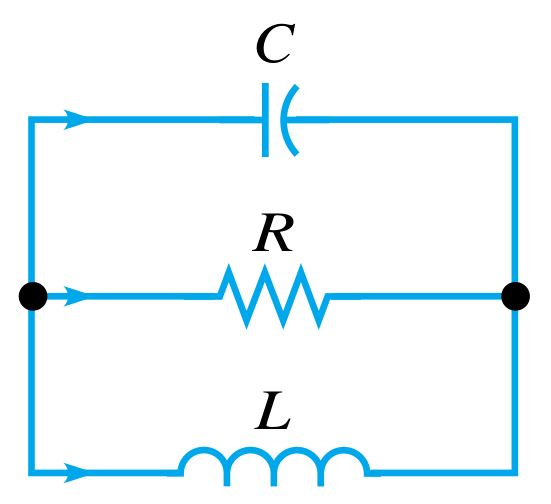
\includegraphics[width=5cm]{circuit}
			\end{center}
			Let $ I_1, I_2, I_3 $ be the currents through the capacitor, resistor, and inductor, respectively. Likewise, let $ V_1, V_2, and V_3 $ be the corresponding voltage drops. The arrows denote an arbitrary positive direction in which current and voltage will be positive. 
			\begin{enumerate}
				\item Applying Kirchoffs second law to the upper loop in the circuit show that \[ V_1 - V_2 = 0 \]
				\item In a similar way show that \[ V_2 - V_3 = 0 \]
				\item Applying Kirchhoffs first law to either node in the circuit show that \[ I_1 + I_2 + I_3 = 0 \] 
				\item Use the current voltage relation to obtain the following 
					\begin{align*}
						CV_1 ' = I_1 && V_2 = RI_2 && LI_3' = V_3
					\end{align*}
				\item Eliminate $ V_2, V_3, I_1, I_2 $ to obtain 
					\begin{align*}
					CV_1 ' = -I_3-\dfrac{V_1}{R} && LI_3' = V_1
					\end{align*}
			\end{enumerate}
		\end{q}
		\begin{q}
			Consider the following circuit 
			\begin{center}
				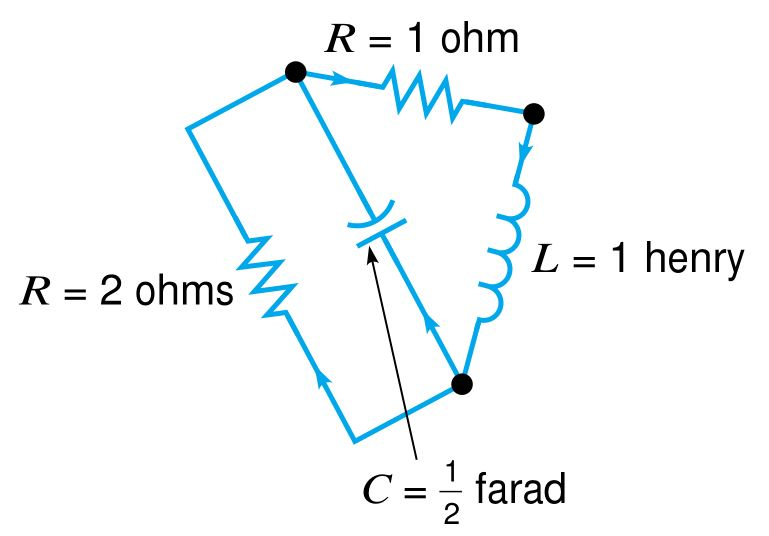
\includegraphics[width=8cm]{circuit2}
			\end{center}
			I will request that you make an honest attempt to do the first step without looking at the second step (cover it up now!!)
			\begin{enumerate}
				\item Express this circuit in terms of a differential system of the form \[ \textbf{x}' = \textbf{Ax} \] 
				\item The answer to the previous question, and the system is given by 
				\[ \dfrac{d}{dt} \left(\begin{matrix} I \\ V \end{matrix}\right) = \left(\begin{matrix} -1 & -1 \\ 2 & -1 \end{matrix}\right) \left(\begin{matrix} I \\ V \end{matrix}\right)   \] Suppose that at time $ t =0 $ the current is 2 amperes and the voltage drop is 2 volts. Find $ I(t) \text{ and } V(t) $ at any time
			\end{enumerate}
		\end{q}
		\begin{q}
			Return back to the circuit we discussed in Question (3)
			\begin{enumerate}
				\item express that circuit in terms of a differential system, similar to the one in Question (4)
				\item show that the eigenvalues are real and equal if $ L = 4R^2C $ 
				\item Suppose that $ R = 1 \Omega, C = 1 F, L = 4H$ Suppose also that $ I(0) = 1 A $ and $ V(0) = 2V $ find $ I(t) \text{ and } V(t) $
			\end{enumerate}
			  
		\end{q}
	\end{multicols*}
\end{document}
